\documentclass[fleqn]{beamer}

% The title of the presentation:
%  - first a short version which is visible at the bottom of each slide;
%  - second the full title shown on the title slide;
\title[DMD-PM]{Acceleration of the Power and Related Methods with Dynamic Mode Decomposition}

% Optional: a subtitle to be displayed on the title slide
%\subtitle{Show where you're from}

% The author(s) of the presentation:
%  - again first a short version to be displayed at the bottom;
%  - next the full list of authors, which may include contact information;
\author[Xu, Reed, Roberts]{Leidong Xu, Richard Reed, Jeremy Roberts}

% The institute:
%  - to start the name of the university as displayed on the top of each slide
%    this can be adjusted such that you can also create a Dutch version
%  - next the institute information as displayed on the title slide
\institute[Kansas State University]{
    Alan Levin Department of Mechanical and Nuclear Engineering\\
    Carl R. Ice College of Engineering \\
    Kansas State University}

% Add a date and possibly the name of the event to the slides
%  - again first a short version to be shown at the bottom of each slide
%  - second the full date and event name for the title slide
\date[ANS W19]{ANS winter meeting 2019}

\usepackage{currfile}
\usepackage{ru}
\usepackage{times}
\usepackage{bm}
\usepackage{graphicx} % allows inclusion of graphics
\usepackage{booktabs} % nice rules (thick lines) for tables
\usepackage{microtype} % improves typography for PDF
\usepackage{tikz}
\usepackage{xcolor}
\usepackage{standalone}
\usepackage{amsmath,amssymb,amsfonts}
\usepackage[]{algorithm2e}
\usepackage[english]{babel}
\usepackage{csquotes}
\usepackage{varwidth}
\usepackage[backend=bibtex, style=authortitle-icomp]{biblatex}
\usepackage{hyperref}
\usetikzlibrary{arrows,shapes}

\newcommand{\SN}{S$_N$}
\newcommand{\mat}[1]{\ensuremath{\bm{#1}}}
\newcommand{\mata}[1]{\ensuremath{\tilde{\bm{#1}}}}
\renewcommand{\vec}[1]{\ensuremath{\bm{#1}}}
\newcommand{\veca}[1]{\ensuremath{\tilde{\bm{#1}}}}
\newcommand{\vd}{\bm{\cdot}} % slightly bold vector dot
\newcommand{\grad}{\vec{\nabla}} % gradient
\newcommand{\ud}{\mathop{}\!\mathrm{d}} % upright derivative symbol
\newcommand{\oper}[1]{\mathcal{#1}}
\providecommand{\e}[1]{\ensuremath{\times 10^{#1}}}
\newcommand{\CHAPTER}[1]{Chapter~\ref{#1}} 
\newcommand{\EQ}[1]{Eq.~(\ref{#1})}               %-- Eq. (refeq)
\newcommand{\EQUATION}[1]{Equation~(\ref{#1})}    %-- Equation (refeq)
\newcommand{\FIG}[1]{Fig.~\ref{#1}}               %-- Fig. refig
\newcommand{\FIGURE}[1]{Figure~\ref{#1}} 
\newcommand{\TAB}[1]{Table~\ref{#1}}              %-- Table tablref
\newcommand{\EQS}[2]{Eqs.~(\ref{#1})--(\ref{#2})}            %-- Eqs. (refeqs)
\newcommand{\EQUATIONS}[2]{Equations~(\ref{#1})--(\ref{#2})}   %-- Eqs. (refeqs)
\newcommand{\EQSTWO}[2]{Eqs.~(\ref{#1})~and~(\ref{#2})}     %-- Eqs. (refeqs)
\newcommand{\EQUATIONSTWO}[2]{Equations~(\ref{#1})~and~(\ref{#2})} 


\makeatletter
\let\beamer@writeslidentry@miniframeson=\beamer@writeslidentry%
\def\beamer@writeslidentry@miniframesoff{%
  \expandafter\beamer@ifempty\expandafter{\beamer@framestartpage}{}% does not happen normally
  {%else
    % removed \addtocontents commands
    \clearpage\beamer@notesactions%
  }
}
\newcommand*{\miniframeson}{\let\beamer@writeslidentry=\beamer@writeslidentry@miniframeson}
\newcommand*{\miniframesoff}{\let\beamer@writeslidentry=\beamer@writeslidentry@miniframesoff}
\makeatother

\addbibresource{bibliography.bib}

\addtobeamertemplate{footnote}{\hskip -2em}{}

\begin{document}
    
\begin{frame}
    \titlepage
\end{frame}

\begin{frame}
    \frametitle{Outline}
    \begin{block}{Presentation Outline}
        \begin{itemize}
            \item K-eigenvalue Problem
            \item DMD-PM(n)
            \item DMD-FPM(n)
            \item Conclusion and Future Work
        \end{itemize}
    \end{block}
\end{frame}

%%%%%%%%%%%%%%%%%%%%%%%%%%%%%%%% introduction    
\section{Background Information}
\begin{frame}{Neutron Transport}
    \begin{block}{Multigroup Neutron Transport Equation}
        \vspace*{-\baselineskip}\setlength\belowdisplayshortskip{0pt}
        \begin{align*}
            \vec{\hat{\Omega}} & \cdot \nabla \psi_g(\vec{r},\vec{\hat{\Omega}}) 
            + \Sigma_{t g}(\vec{r}) \psi_{g}(\vec{r},\vec{\hat{\Omega}}) \\
            &= \frac{1}{4\pi} \sum\limits^{N_g}_{g'=1} \Sigma_{s g g'}(\vec{r}) \phi_{g'}(\vec{r})
            + \frac{\chi_g}{4\pi k} \sum\limits^{N_g}_{g'=1} \nu\Sigma_{fg'}(\vec{r}) \phi_{g'}(\vec{r}) 
        \end{align*}
    \end{block}
    \begin{block}{Operator Notation}
        \vspace*{-\baselineskip}\setlength\belowdisplayshortskip{0pt}
        \begin{equation*}
            \mat{L} \vec{\psi} = \mat{M}\mat{S}\vec{\phi} + \frac{1}{k}\mat{M}\mat{F}\vec{\phi}
            \quad\text{where}\quad
            \vec{\phi} = \mat{D}\vec{\psi}
        \end{equation*}
        \begin{equation*}
            \left(\mat{I} - \mat{D}\mat{L}^{-1}\mat{M}\mat{S}\right) \vec{\phi} = \frac{1}{k} \mat{D}\mat{L}^{-1}\mat{M}\mat{F} \vec{\phi}  
        \end{equation*}
        \begin{equation*}
            \mat{A} \vec{x} = \frac{1}{k} \mat{B} \vec{x}  
        \end{equation*}
    \end{block}
\end{frame}    

\begin{frame}{Power Method}
    \begin{block}{PM Algorithm}
        \begin{algorithm}[H]
            \DontPrintSemicolon
            \KwIn{Material properties and geometry}
            initialize scalar flux $\mathbf{\phi}^{0}$, eigenvalue $k$, $i=1$ \;
            \While{RHS not converged}{
                compute fission source, i.e., \vec{b} = $\frac{1}{k} \mat{D}\mat{L}^{-1}\mat{M}\mat{F} \vec{\phi}^{i-1}$\;
                \While{LHS not converged}{
                    compute scattering source, i.e.,  $\left(\mat{I} - \mat{D}\mat{L}^{-1}\mat{M}\mat{S}\right)\vec{\phi}^{i}= \vec{b}$\;
                }
                update eigenvalue $k$ and normalize eigenvector $\vec{\phi}^{i}$\;
                set i = i + 1
            }
            \KwResult{dominant eigenvalue and steady-state neutron flux}
        \end{algorithm}
    \end{block}
\end{frame} 

\begin{frame}{Dynamic Mode Decomposition}
    A sequential dataset ($\mathbf{X} \subseteq \mathbb{R}^{n\times m}$) spaced by $\Delta t$.\footnotemark
    \begin{figure}[!htb]
        \centering
        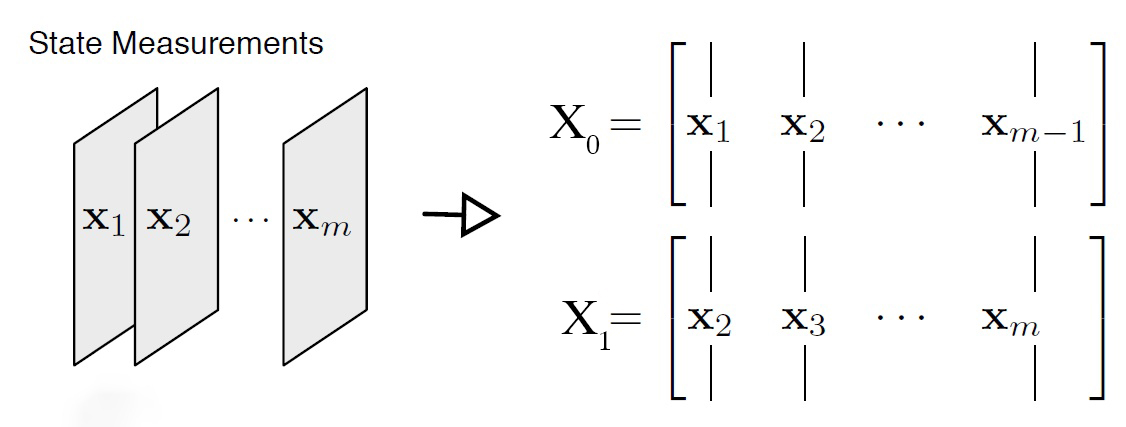
\includegraphics[scale=0.17]{figures/snapshot.jpg}
    \end{figure} 
    \small{\textbf{Assumption}}: 
    $\vec{X}_1 \approx \mat{A} \vec{X}_0$
    \footnotetext{\cite{schmid_dynamic_2010}}
    \footnotetext{\cite{schmid_applications_2011}} 
\end{frame}

\begin{frame}{Dynamic Mode Decomposition}
    \begin{block}{Algorithm}
        \begin{enumerate}
            \item Compute reduced SVD decomposition of $\mat{X}_0 \approx \mat{U}_r \boldsymbol{\Sigma}_r \mat{V}_r^*$
            \pause
            \item Compute $\mata{A}=\mat{U}_r^*\mat{A}\mat{U}_r=\mat{U}_r^*\mat{X}_1\mat{V}_r\boldsymbol{\Sigma}_r^{-1}$
            \pause
            \item Compute the eigendecomposition $\mata{A}=\veca{W}\boldsymbol{\Lambda}\veca{W}^*$
            \pause
            \item Calculate the DMD modes as ${\boldsymbol{\Phi}}=\mat{X}_1\mat{V}_r\boldsymbol{\Sigma}_r^{-1}\mata{W}$
            \pause
            \item Compute the continuous eigenvalues $\omega_i = \log(\frac{\lambda_i}{\lambda_0}) / \Delta t$
            \pause
            \item Compute $\vec{b}=\boldsymbol{\Phi}^\dag \vec{x}_0$
            \item Predict the response by $\vec{x}^\text{DMD}(t) = \sum\limits_{i=0}^r\vec\phi_0\exp(\omega_i t)b_i=\boldsymbol{\Phi}\exp(\boldsymbol\Omega t)\vec{b}$
        \end{enumerate}
    \end{block}
\end{frame}

\begin{frame}{Modified DMD Algorithm for the NTE \footnotemark}
    \begin{block}{}
        Reminder
        \begin{equation*}
            \vec{x}^\text{DMD}(t) \approx \sum^{r}_{i=1} \vec{\phi}_i \exp(\omega_i t) b_i = \boldsymbol{\Phi}\exp(\boldsymbol\Omega t)\vec{b} \, 
        \end{equation*}
        Power method leads to a single dominant mode, i.e.,
        \begin{equation*}
            \lim\limits_{t\rightarrow\infty}\vec{\phi}_i \exp(\omega_i t) b_i = 0 \quad\forall\quad i > 1
        \end{equation*}
        Thus,
        \begin{equation*}
            \vec{x}^{DMD}(\infty) = \vec{\phi}_0 b_0 
        \end{equation*}
    \end{block}
    \footnotetext[2]{\cite{roberts2019acceleration}}
\end{frame} 

\begin{frame}{} % Objective
    \begin{block}{Objective}
        Estimate accurate fundamental eigenmodes using DMD to accelerate the power method and other, related methods resulting in:
        \begin{itemize}
            \item Faster convergence
            \item Lower computational cost
        \end{itemize}
    \end{block}
\end{frame}

%%%%%%%%%%%%%%%%%% DMD-PM
\section{Methods}
% \begin{frame}{DMD-PM(n)}
%     \begin{block}{Algorithm}
%         \begin{enumerate}
%             \item Guess $\vec{x}^{(0)}$ and normalize.
%             \pause
%             \item Perform $n$ power iterations to produce $\mat{X}_0$ and $\mat{X}_1$
%             \pause
%             \item Compute the DMD modes through rth-order 
%             \pause
%             \item Estimate $\vec{x}^{(\infty)}=\vec{x}(\infty)$
%             \pause
%             \item Set $\vec{x}^{(0)}$ as normalized $\vec{X}^{(\infty)}$  
%             \pause
%             \item Return to steps 1 until convergence
%         \end{enumerate}
%     \end{block}
% \end{frame}  

%%%%%%%%%%%%%%%%%% Flattened Power Method
\begin{frame}{Transport Operators}
    \begin{block}{Neutron Transport Equation}
        \vspace*{-\baselineskip}\setlength\belowdisplayshortskip{0pt}
        \begin{equation*}
            \vec{\phi} - \mat{D}\mat{L}^{-1}\mat{M}\mat{S}\vec{\phi} = \frac{1}{k} \mat{D}\mat{L}^{-1}\mat{M}\mat{F} \vec{\phi}  
        \end{equation*}
    \end{block}
    \begin{block}{Power Method Operator}
        \vspace*{-\baselineskip}\setlength\belowdisplayshortskip{0pt}
        \begin{equation*}
            \vec{\phi}^{i} = \left(\mat{I} - \mat{D}\mat{L}^{-1}\mat{M}\mat{S}\right)^{-1} \left(\frac{1}{k} \mat{D}\mat{L}^{-1}\mat{M}\mat{F}\right) \vec{\phi}^{i-1} 
        \end{equation*}
    \end{block}
    \begin{block}{Flattened Power Method Operator\footnotemark}
        \vspace*{-\baselineskip}\setlength\belowdisplayshortskip{0pt}
        \begin{equation*}
            \vec{\phi}^{i} =  \mat{D}\mat{L}^{-1}\mat{M} \left(\mat{S} + \frac{1}{k} \mat{F}\right)\vec{\phi}^{i-1}   
        \end{equation*}
    \end{block}
    \footnotetext{\cite{gill_newtons_2011}}
\end{frame}  

\begin{frame}{Method Comparison}
    \begin{columns}[T]
        \begin{column}{0.5\linewidth}
            \begin{block}{PM Algorithm}
                \begin{algorithm}[H]
                    \DontPrintSemicolon
                    \KwIn{Material properties}
                    initialize $\vec{\phi}^{0}$, $k$, $i=1$\;
                    \While{RHS unconverged}{
                        compute fission source\;
                        \While{LHS unconverged}{
                            compute scatter source\;
                        }
                        update $k$\;
                        normalize $\vec{\phi}^{i}$\;
                        set i = i + 1
                    }
                    \KwResult{dominant k and \vec\phi}
                \end{algorithm}
            \end{block}
        \end{column}
        \begin{column}{0.5\linewidth}
            \begin{block}{FPM Algorithm}
                \begin{algorithm}[H]
                    \DontPrintSemicolon
                    \KwIn{Material properties}
                    initialize $\vec{\phi}^{0}$, $k$, $i=1$\;
                    \While{unconverged}{
                        compute fission source\;
                        compute scatter source\;
                        update $k$\;
                        normalize $\vec{\phi}^{i}$\;
                        set i = i + 1
                    }
                    \KwResult{dominant k and \vec\phi}
                \end{algorithm}
            \end{block}
        \end{column}
    \end{columns}
\end{frame} 

\begin{frame}{Recovering the eigenvalue from DMD}
    \begin{block}{Trouble predicting k}
        \begin{itemize}
            \item DMD uses snapshots of the normalized $\phi$
            \item DMD predicts a normalized $\phi$
            \item No way to to retrieve k without another sweep
        \end{itemize}
    \end{block}
    \pause
    \begin{block}{Use Aitken Extrapolation for a better prediction of $k^{(\infty)}$ \footnotemark}
        \vspace*{-\baselineskip}\setlength\belowdisplayshortskip{0pt}
        \begin{equation*}
            k_{aitken} = k^{(i-2)} - \frac{(k^{(i-1)}-k^{(i-2)})^2}{(k^{(i)} - 2k^{(i-1)} + k^{(i-2)})}
        \end{equation*}
    \end{block}
    \only<2>\footnotetext{\cite{aitken_1927}}
\end{frame}

\begin{frame}{DMD algorithm for (flattened) power method}
    \begin{block}{Algorithm}
        \begin{enumerate}
            \item Assume $k^{(0)}$, $\vec\phi^{(0)}$ and normalize
            \pause
            \item Perform $n$ applications of the (flattened) operator
            \pause
            \item Form $\mat{X}_0$ and $\mat{X}_1$ from snapshots of $\vec\phi$
            \pause
            \item Compute the DMD modes $b$
            \pause
            \item Predict converged solution $\vec\phi^{(\infty)}$
            \pause
            \item Update $k$ by Aitken extrapolation
            \pause
            \item Return to step 1 until converged
        \end{enumerate}
    \end{block}
\end{frame}   

\section{Results}
\begin{frame}{2-D, 2-group IAEA Diffusion Benchmark\footnotemark}
    \begin{figure}
        \centering
        \includestandalone[mode=buildnew,height=0.6\paperheight]{figures/iaea2d}
    \end{figure}
    \footnotetext[5]{\cite{center1977benchmark}}
\end{frame}

\begin{frame}{IAEA 2-D diffusion}
    \begin{figure}
        \centering
        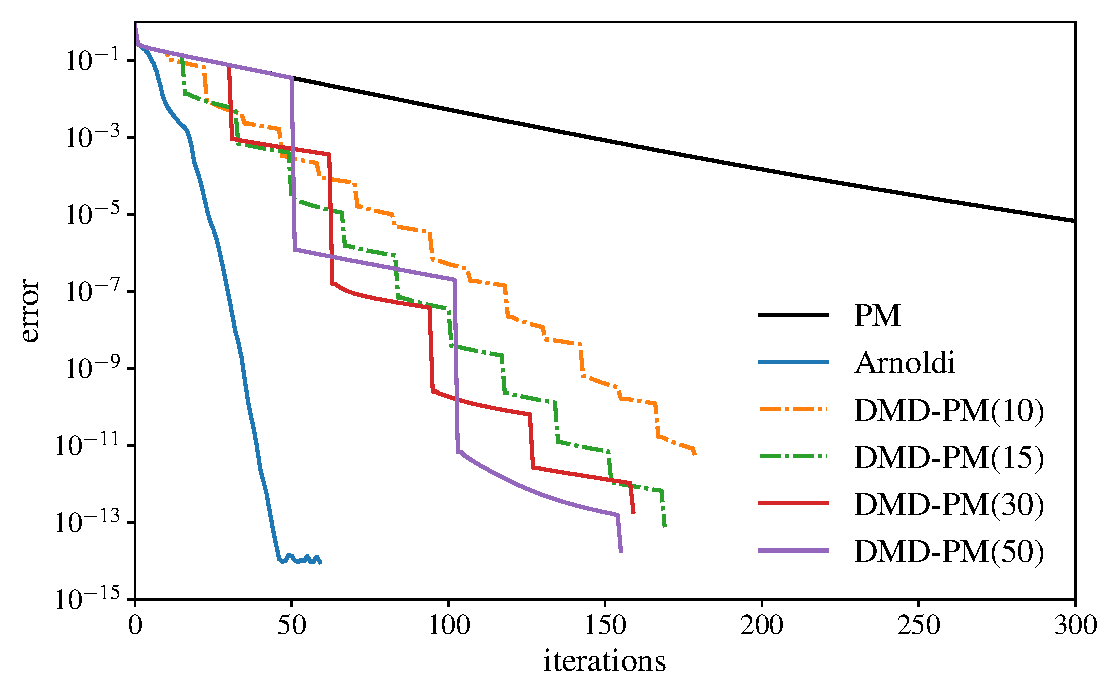
\includegraphics[height=0.69\paperheight]{figures/dmdpi_semilog.pdf}
    \end{figure}
\end{frame}

\begin{frame}{Configuration of 1-D Boiling Water Reactor \footnotemark}
    \begin{figure}
        \centering
        \begin{minipage}[c]{\textwidth}
            \centering
            \includestandalone[mode=buildnew, width=1.0\linewidth]{figures/core1}
        \end{minipage}
        \begin{minipage}[c]{\textwidth}
            \centering
            \includestandalone[mode=buildnew, width=0.4\linewidth]{figures/assemblies}
        \end{minipage}
        \begin{minipage}[c]{\textwidth}
            \centering
            \includestandalone[mode=buildnew, width=0.8\linewidth]{figures/core_materials}
        \end{minipage}
    \end{figure}
    \begin{itemize}
        \item 18 mesh cells per fuel region
        \item 6 mesh cells per moderator region
    \end{itemize}
    \footnotetext[6]{\cite{rahnema_generalized_2008}}
\end{frame}

\begin{frame}{1-D Boiling Water Reactor Test}
    \begin{figure}
        \centering
        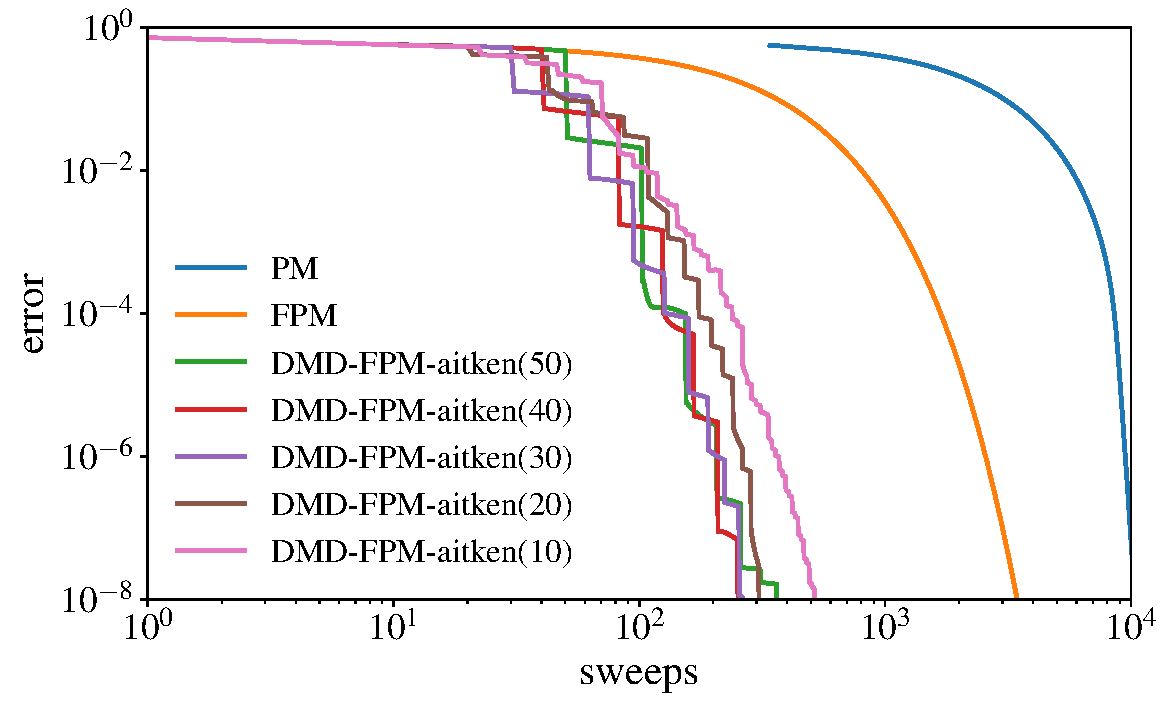
\includegraphics[height=0.65\paperheight]{figures/dmd_ospi_loglog_1d.pdf}
    \end{figure}
\end{frame}

\begin{frame}{Configuration for the C5G7 benchmark\footnotemark}
    \begin{figure}
        \centering
        \includestandalone[mode=buildnew,height=0.6\paperheight]{figures/C5G7_config}
    \end{figure}
    \footnotetext[7]{\cite{oecd_nuclear_energy_agency_benchmark_2003}}
\end{frame}

\begin{frame}{Assembly Configurations}
    \begin{columns}[c]
        \begin{column}{.45\textwidth}
            \begin{figure}
                \centering
                \includestandalone[mode=buildnew,width=\linewidth]{figures/UO2_config}
            \end{figure}
        \end{column}
        \begin{column}{.45\textwidth}
            \begin{figure}
                \centering
                \includestandalone[mode=buildnew,width=\linewidth]{figures/MOX_config}
            \end{figure}
        \end{column}
    \end{columns}
\end{frame}

\begin{frame}{2-D C5G7}
    \begin{figure}
        \centering
        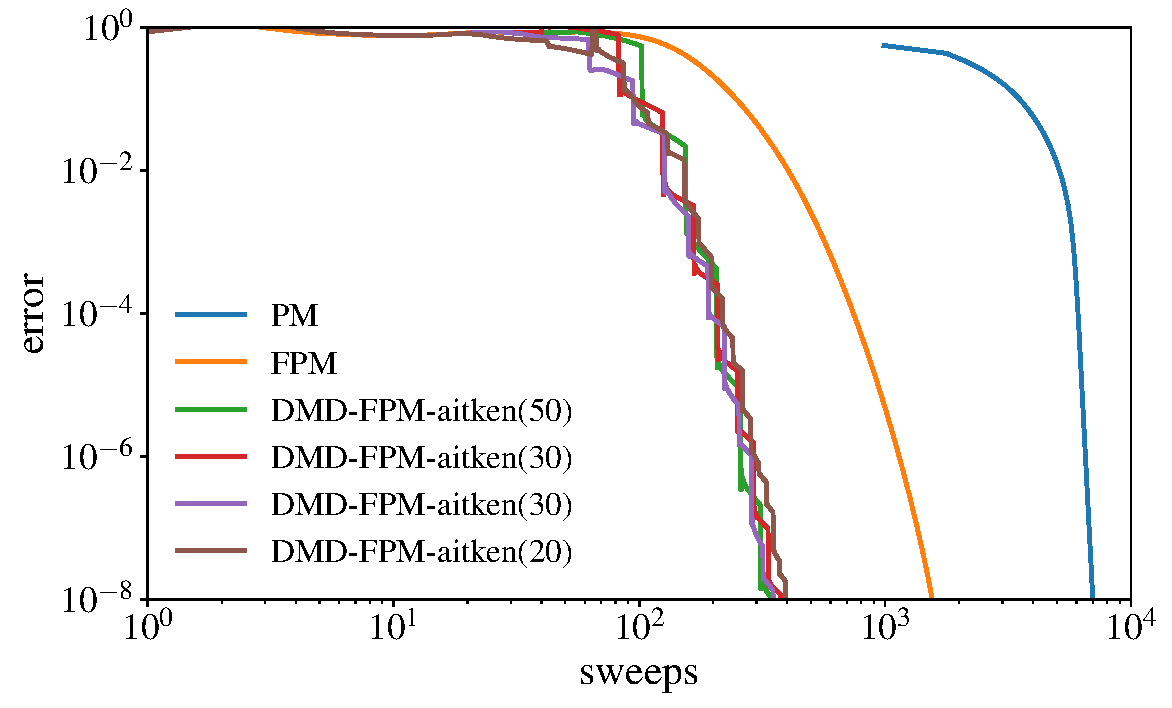
\includegraphics[height=0.65\paperheight]{figures/dmd_ospi_loglog_c5g7_new.pdf}
    \end{figure}
\end{frame}

\section{Conclusions and Future Work}
\begin{frame}{Conclusions and Future Work}
    \begin{block}{Conclusions}
        \begin{enumerate}
            \item 5x speedup for DMD-PM(n)
            \item 5x-10x speedup for DMD-FPM(n)
        \end{enumerate}
    \end{block}
    \begin{block}{Future Work}
        \begin{enumerate}
            \item Acceleration of Monte Carlo Method 
            \item Accurate Estimation of Eigenvalue for the flattened Power Method 
        \end{enumerate}
    \end{block}
\end{frame}  

\end{document}
